\anexo{Cronograma de Actividades}

Durante el desarrollo del proyecto, se realizó un ajuste en la planificación inicial vinculada a las etapas de relevamiento y validación. Originalmente, se había previsto iniciar la recolección de información mediante encuestas estructuradas. Sin embargo, en función de las necesidades emergentes del proyecto y con el objetivo de alcanzar una comprensión más profunda del contexto real, así como detectar patrones y problemáticas concretas del rubro gastronómico, se optó por priorizar una instancia cualitativa basada en entrevistas semiestructuradas. 

Como parte de esta decisión, se amplió la cantidad de entrevistas relevadas y por ende la duración de las mismas, incluyendo la transcripción y el análisis de dichas representaciones del sector.

Como consecuencia, la encuesta fue reprogramada para una segunda instancia, a fin de que las preguntas formuladas reflejen con mayor precisión los escenarios identificados, todo esto con el fin de favorecer una toma de decisiones más informada a lo largo del desarrollo del proyecto.

\begin{figure}[ht]
    \centering
    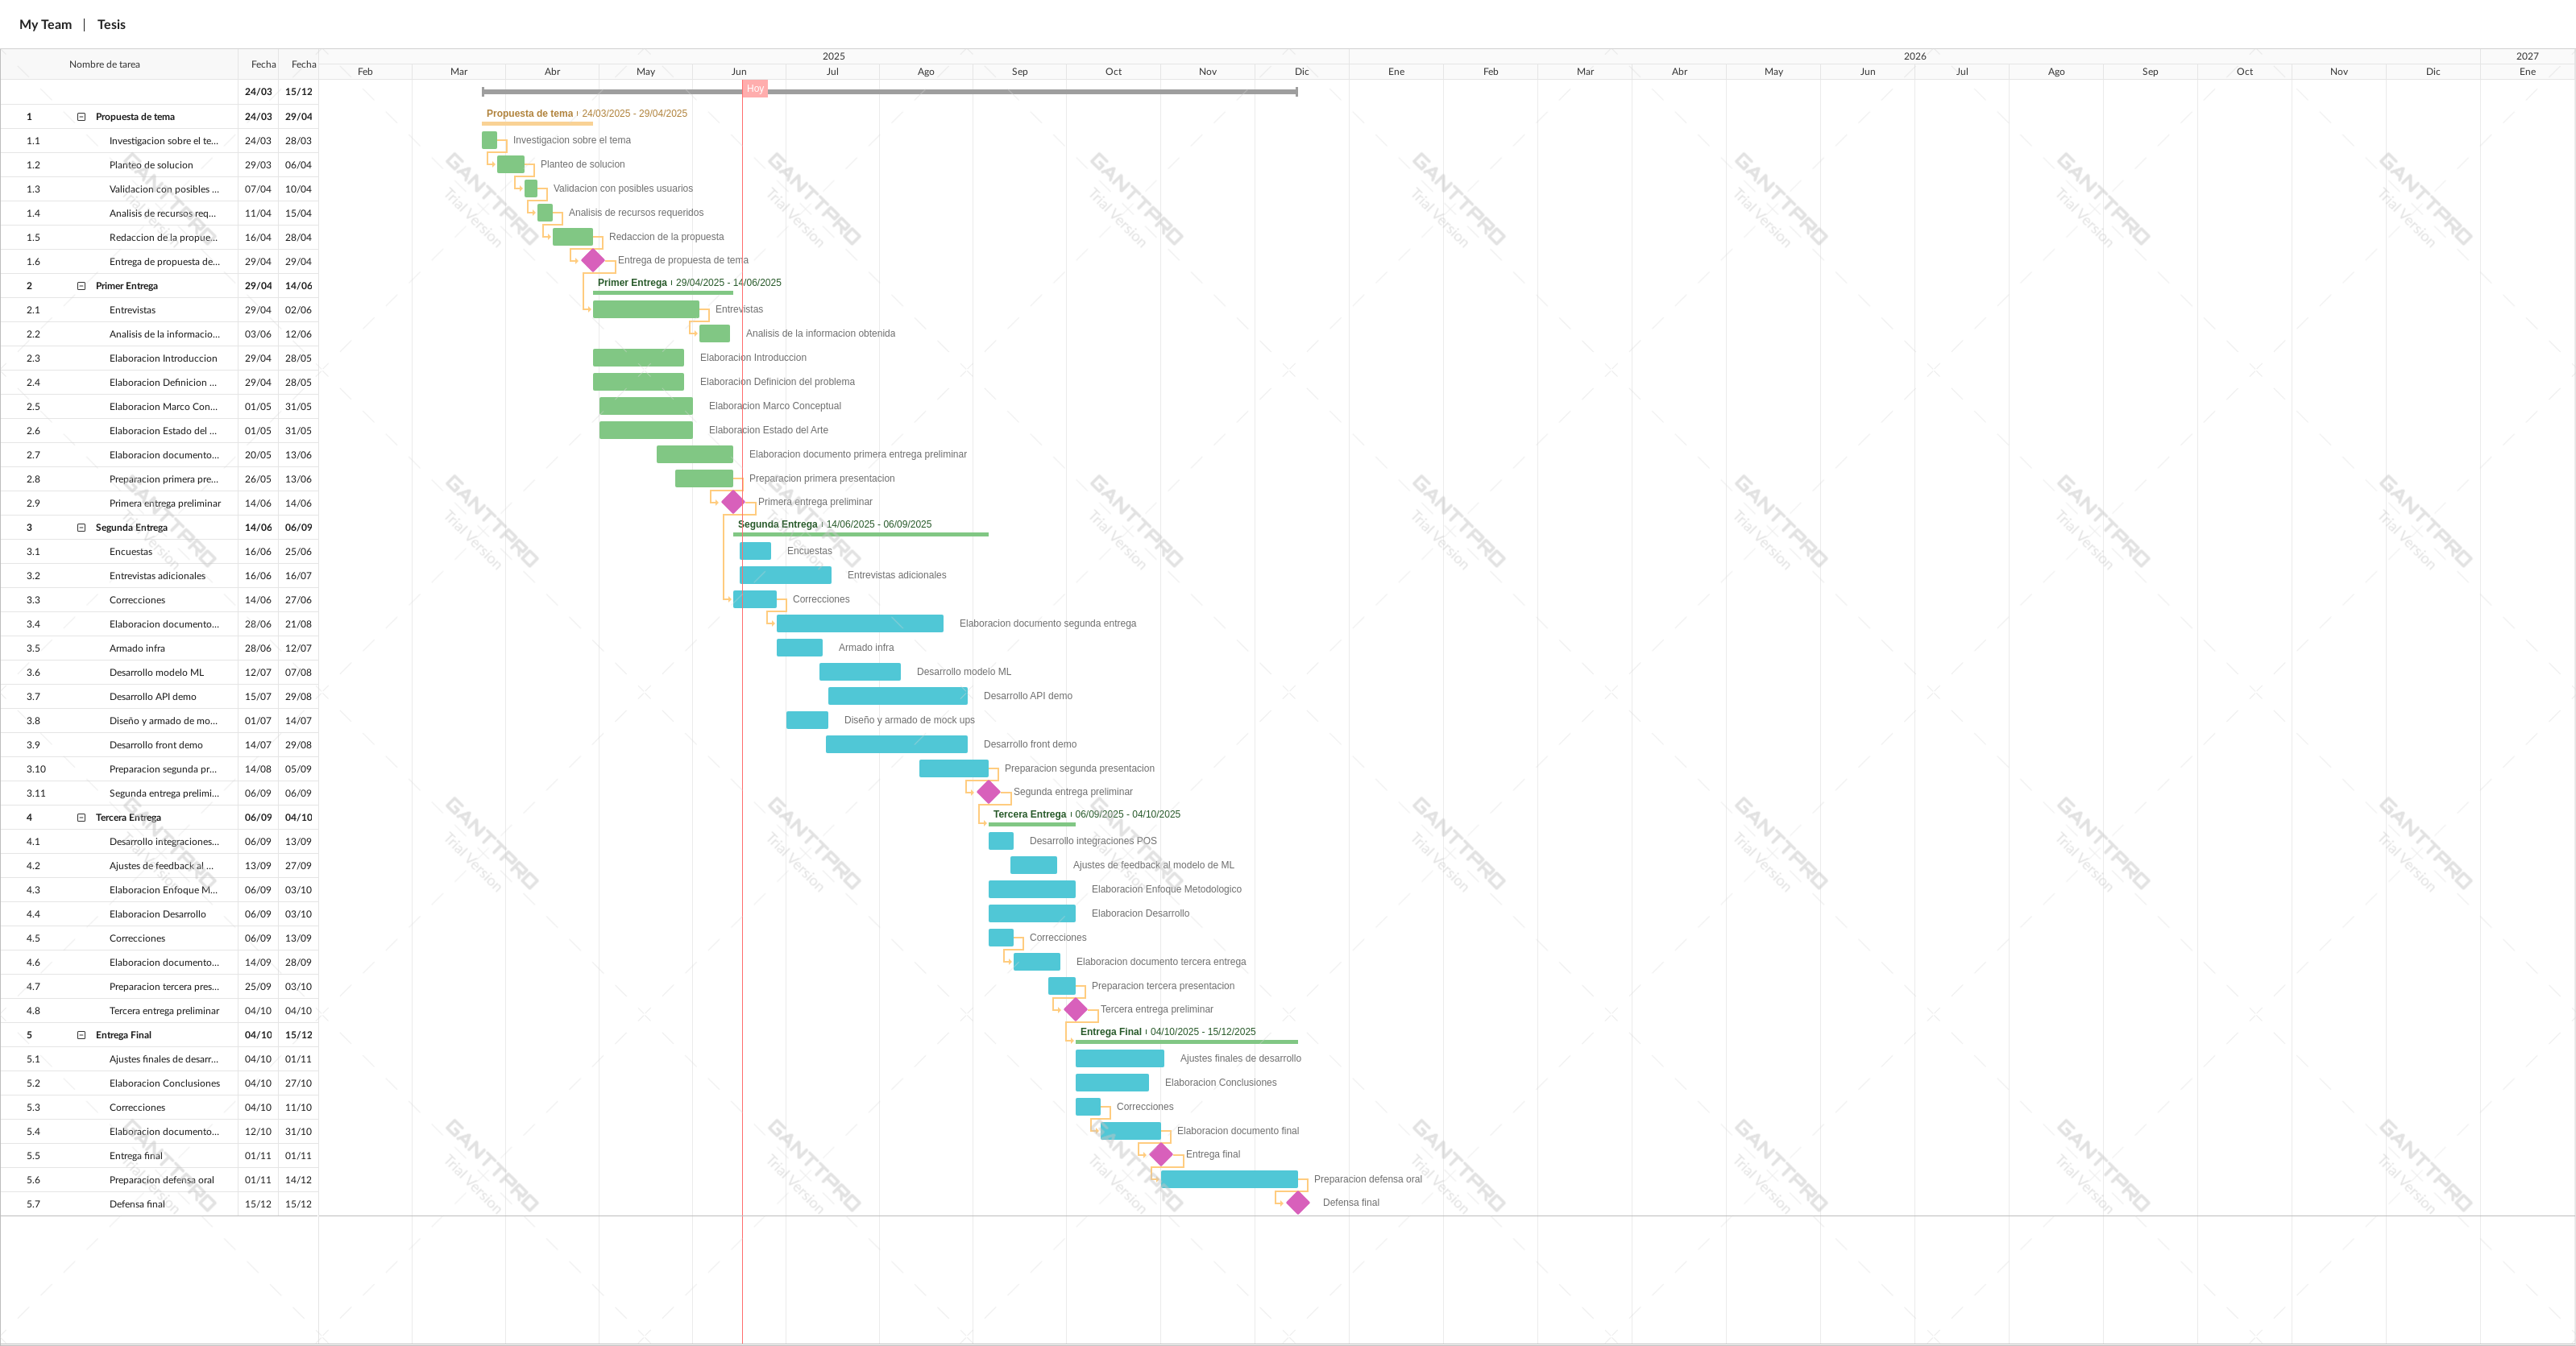
\includegraphics[width=0.7\textwidth]{images/cronograma.png}
    \caption{Cronograma actualizado de actividades.}
    \label{fig:cronograma}
\end{figure}
